
\begin{figure}[t!]
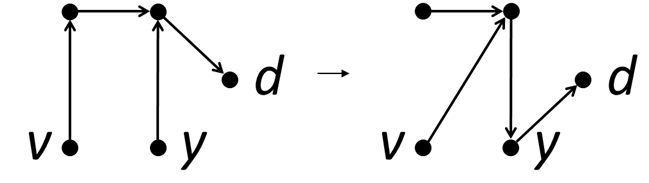
\includegraphics[width=3in]{figures/noloops.png}
\caption{Example scenario discussed in \S\ref{sec:example}. \ratul{better figures?}]
}
\label{fig:example}
\end{figure}

\section{Loop Freedom}
\label{sec:loop-free}

To expose the nuances of updating SDNs while maintaining consistency, we focus in this section on a basic, natural consistency property---loop freedom. As the name suggests, it refers to the property that no packet should loop in the network.  In the next section, we will analyze a broader set of consistency properties.

Consider the five-node network in Figure \ref{fig:example}. Assume that we want to update the routing to Node $d$ from the pattern on the left to that on the right. A naive way to update is to simply send out the forwarding updates (e.g., ask $v$ to send packets destined to $d$ to $x$.). However, during application of these updates, it might happen that $x$ updates its rule before $y$, introducing a routing loop between $x$ and $y$. This loop will eventually disappear, once $y$ updates its rule, but in an asynchronous system, with possible message delays and losses, it is difficult to guarantee when this will happen.

Reitblatt et al.~\cite{safeupdates} proposed an update procedure that can provide loop freedom. It  relies on ingress nodes stamping packets with version numbers, by encapsulating them in another header. Assume that the version being currently stamped is $k.$ Then, the update procedure works as follows: $i)$ send new rules at each node applicable to packets with version $k+1$; $ii)$ after all nodes have acknowledged that they have updated, ask the ingress nodes to switch to stamping version $k+1$; $iii)$ after waiting for a time during which all version $k$ packets should have left the network, delete the old rules.

%If the old and the new rule sets are loop free, this procedure guarantees loop freedom during updates because version $V$ packets always use old rules and version $V+1$ packets always use new rules. Note, however, that new rules only start getting used in the second step, after all nodes have been updated.

%At the other end of the spectrum, the SDN controller could first (i) distribute the new rules, then (ii) wait for an acknowledgement of all the nodes that they have received the new rules, then (iii) tell all the nodes to stop sending packets, and finally, once (iv) they all acknowledged that, (v) tell the nodes to now use the new rules. After the nodes (vi) acknowledge that they are using the new rules, the SDN controller can tell them to (vii) remove the old rules, as they are not needed anymore. This solution does not suffer from loops, as the old and the new solution are well-separated in time.\footnote{Strictly speaking, this protocol is not sufficient, as there might be packets in transit, still using the old rules when rushing through the protocol. Consider a packet sent from sent from $y$ to $x$ shortly before $y$ received the order to stop sending (iii). If node $x$ already passed the last step of the protocol when receiving the packet, node $x$ has not other option then sending the packet back to node $y$, i.e. the packet is experiencing a loop.} However, it is also terribly slow. One may speed up the process by omitting steps (iii) and (iv). Now, assuming that node $x$ received the command to use the new rule (v) earlier than node $y$. As such, in order to guarantee no loop between nodes $x$ and $y$, we must introduce version numbers in packets such that nodes $x$ and $y$ know that packets from $x$ respectively $y$ must be treated according to the new respectively old rules. This is the solution proposed by \cite{theoriginalprincetonpaper}.

%One may ask whether version numbers are really necessary, just to guarantee no loops? Also, one may ask whether a faster solution is possible. What nodes are really dependent on each other? This may look like a technicality, but as we all know, nodes are often temporarily unavailable or reacting slowly. If a node must wait for another node, there should better be a consistency reason for it, and not merely protocol overhead. Is there something like a \emph{minimal protocol for a given consistency guarantee}? This is exactly the question we address in this paper.

The procedure above is onerous---it requires that all nodes be updated (in step $i$) before new rules become usable (in step $ii$), which means that delays in updating even one node will delay the update, and it requires additional headers in packets. However, it also guarantees a consistency property that is stronger than loop freedom---each packet is routed entirely using the old rules or the new rules, and never a mix of the two sets. We call this property packet coherence in \S\ref{sec:table}.

Now, a natural question is: if we want only loop freedom (not packet coherence), can we design an update procedure that does not rely on updating all nodes before starting to use any of the new forwarding rules?  This is not a technicality, as nodes in a production network can often react slowly, or they may even be temporarily unreachable via the controller~\cite{b4}.  Thus, solutions in which the network can quickly start using as many of the new forwarding rules as possible, while maintaining consistency property of interest, are preferable.

A related, fundamental question is: for a given consistency property of interest, what is the minimal procedure. This is the question we raise in this paper. While the next section contains a broader discussion, returning to loop freedom, we describe below two update procedures, both of which have looser dependency requirements than Reitblatt et al.'s procedure.  The first of these is simpler and the second is in fact minimal.

%To gain intuition underlying this procedure, observe in our example that $u$ does not even need to change its rule, as it always just forwards to $x$. Hence, it does not even have to be informed about the rule changes. Further, $v$ can switch immediately, as irrespective of the rules being used by other nodes, the packet will end up at $x$, with no possibility to experience a loop. Node $y$ can also switch immediately to the new rule, as its packet will then directly reach the destination $d$. The only critical node is $x$, which must wait until $y$ implements the switch; otherwise the network might experience a loop.


\subsection{A simple procedure}
\label{sec:practical}

%(Assume for now that rules correspond to unique destinations, as in tunnel-based routing. We discuss later rules that have overlapping destinations, as in prefix-based routing.)

Our procedure can be understood in terms of a {\em dependency tree} in which a node can safely switch to using new rules after its parent has switched. Thus, a given node only depends on its ancestors for switching, and any slowdowns elsewhere in the network have no impact on its ability to switch. A simple, valid dependency tree is basically the destination rooted in-tree with respect to the new set of rules. For simplicity, we first describe our procedures as if there was just a single destination $d$, and then later discuss the case of multiple destinations. In this tree, the destination is the root, and a node $c$ is a child of $p$ iff the new rule of $c$ points to $p$. In our example, this is basically the tree shown on the right in Figure \ref{fig:example}.

A simple update procedure is then as follows: starting with the root of a destination-rooted dependency tree, successively update the children, pursuing the branches in parallel.
%Update dependency trees of different destinations in parallel, and for a given tree, update children of a node in parallel.
It is easy to see that this procedure guarantees loop freedom: Nodes that are in the dependency tree of the destination will only switch to the new rule once all the nodes on the new path to the destination have already switched.

%However, based on the discussion on the example, it is easy to see that this solution is not minimal, as node $v$ cannot switch immediately, after learning the new rule, but must wait on $x$.



%More generally, loop freedom requires rule updates to wait for each other in a \emph{dependency tree}, i.e., a node may have to wait for one parent node having switched to the new rule before being able to switch itself. A simple dependency tree works as follows: Let the destination $d$ be the root of the dependency tree. A node $c$ is a child of parent $p$ in the dependency tree if and only if the new rule of $c$ points to $p$. In Figure \ref{fig:example}, $x$ is a parent of $u$ and $v$.

%Now, starting at the root of the dependency tree, nodes first switch to the new rule, and then inform all their children in the dependency tree to switch as well. Apart from the packets-in-transit problem described in footnote 1 (TODO), correctness is immediate:



\begin{figure}[t!]
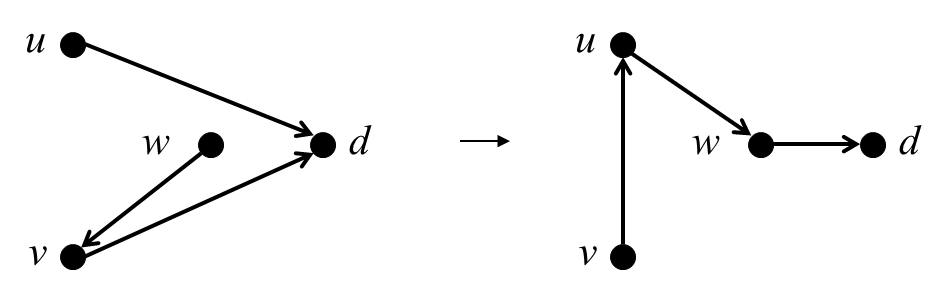
\includegraphics[width=3in]{figures/nominimum.png}
\caption{Example with two orthogonal minimal solutions, discussed in Section \ref{sec:minimal}.}
\label{fig:minimal}
\end{figure}

\subsection{A minimal procedure}
\label{sec:minimal}

%In Section \label{sec:minimal}, we will show a slightly more complicated algorithm which produces a minimal result that can also be computed in polynomial time.

While correct, the procedure above is not minimal. Observe that $v$ can switch to new rules immediately, irrespective of whether $x$ (its parent in the destination tree) is updated; no matter what, packets will end up at $x$, with no possibility to experience a loop.

One may wish for the fastest procedure, in the sense that dependencies are minimum. Surprisingly, this is not trivial. Consider the example network in Figure~\ref{fig:minimal}, again with the old rules on the left, and the new rules on the right. Node $w$ may switch to the new rule immediately, but not nodes $u$ and $v$. If they both switch immediately, and $w$ is still using the old rule, we get a loop. So, one of them must wait for $w$ to switch. However, either one is fine, i.e. either $u$ must wait for $w$ (and $v,w$ may switch immediately), \emph{or} $v$ must wait for $w$ (and $u,w$ may switch immediately). In other words, there are two valid dependency trees, one which is fast for node $u$ (at the expense of node $v$), and one which is fast for node $v$ (at the expense of node $u$).
This example shows that \emph{the minimum} solution does not exist, and we must look for \emph{a minimal} solution instead. A minimal solution is one in which no node can improve its dependencies without some other node getting worse.

In designing such a solution, we observe that there may be many nodes that can switch immediately. For example, in Figure \ref{fig:example}, nodes $v$ and $y$ can switch immediately, for different reasons. We thus expand the concept of a dependency tree into a \emph{dependency forest}. As before, children wait for their parents before switching to new rules, but we now have multiple roots and trees. Our goal is to look for a minimal dependency forest, in the sense that one cannot remove a subtree of the forest with subtree root $c$ (and parent $p$) and re-attach it at an ancestor of $p$, or make $c$ a root of the forest.

In our algorithm, each node is in one of three states, \emph{old}, \emph{new}, or \emph{limbo}, depending on whether the node is guaranteed to only use its old rule or new rule, or whether it might use both rules, respectively. Since the destination $d$ does not have any rules, neither old nor new, it is by definition in state new.

We construct the dependency forest as follows: We start out with only the old rules, by definition a loop-free in-tree to destination $d$. Now, for each node $u$, we test whether adding $u$'s new rule will introduce a loop, using a loop-detection subroutine (described below). If not, node $u$ is entering the state limbo, and added as a root in the dependency forest. On the other hand, if $u$'s new rule introduces a loop, node $u$ remains old, and must wait until we find its parent in the dependency forest. The initialization is completed after we processed all the nodes, and found all the roots (which are now leaves in our incomplete dependency forest). Next we add the children to the dependency forest, one after another. In each step, we choose a limbo (dependency forest leaf) node $u$. We remove $u$'s old rule from the network (putting $u$ in the new state), and then check upon all the old nodes, trying to find nodes $v$ where the new rule of $v$ does not introduce a loop (using the same loop-detection subroutine), thanks to removing $u$'s old rule. If we find such a node $v$, then node $v$ is a child of $u$ in the dependency forest, and a new leaf of the dependency forest, in limbo state. If no such node $v$ exists, node $u$ remains a childless leaf of the dependency forest. It may happen that we find no more limbo node, that is, all nodes are either new or old. In this case, as proved below, we will always find an old node that can become new directly.
We continue until we processed all nodes in the network.

The loop-detection subroutine can be implemented in various ways, for instance by using
%the Kosaraju-Sharir algorithm or
Tarjan's algorithm \cite{tarjan72}. As Tarjan's algorithm does not only detect loops, but finds strongly connected components, let us briefly describe a simpler solution for loop-detection here: Our loop-detection subroutine is a simple recursive procedure, starting at the new rule $u.new = v$. Nodes are in one of three states, unknown, seen, and visited. Both Nodes $u,v$ are seen, all other nodes are unknown. Now we do a depth-first search (DFS), starting at $v$. If the DFS visits a Node $w$, depending on the state of $w$, we do the following: If $w$ is unknown, we mark $w$ as seen and continue the DFS. If $w$ is visited, we backtrack the DFS. If $w$ is seen, we found a loop and stop. When backtracking to Node $w$, we mark $w$ as visited. If the DFS does not find a loop, and we backtrack all the way to the starting node $v$, the network is loop-free, and we can safely add the new rule.


%Clearly, the order in which the nodes are visited will determine the dependency forest, however, irrespective of the order is, the dependency tree is minimal (see below).

%TODO: alternative formulation, shorter, maybe better: Initially, we let all good nodes to be roots of the dependency forest. Then, iteratively, while not all nodes are processed, we process an arbitrary good node $u$ by removing its old rule. Removing $u$'s old rule might turn other nodes good; if $v$ turns good when processing $u$, then $v$ is a child of $u$ in the dependency forest.

Once a dependency forest is computed, we update the individual dependency trees in parallel. For this procedure above, we can prove that the computed dependency forest is correct (that is, applying updates based on them guarantees loop-freedom) and minimal. We include the proofs in the Appendix. Regarding efficiency, the loop-finding subroutine can be done in linear time. Since we must process each node, and check for each not yet processed node when doing so, the total time of the algorithm is cubic in the size of the network.\footnote{We suspect that this running time can be improved, but this is beyond the scope of this paper.}

\subsection{Multiple destinations}
\label{sec:multidest}

While we described the procedures above in terms of a single destination node, their correctness and optimality properties hold in the presence of multiple destinations as long as rules are per-destination. This setting maps to layer 2 routing, which uses MAC addresses as destinations, or tunnel-based routing, which users tunnel identifiers as destinations. (The two large-scale SDNs described in recent literature use tunnel-based routing~\cite{swan,b4}.) Here, we can compute dependency trees or forests for each destination separately and apply updates in parallel.

\begin{figure}[t!]
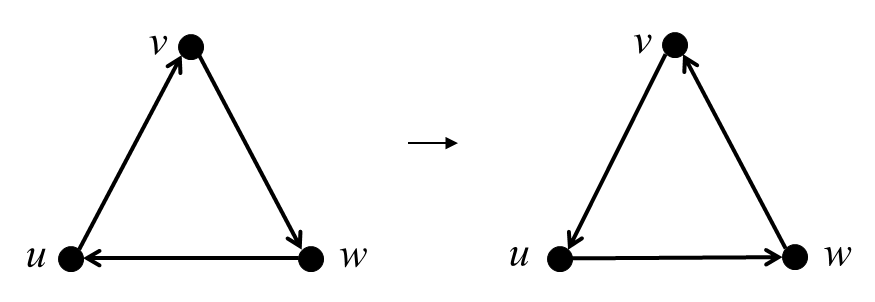
\includegraphics[width=3in]{figures/multidest.png}
\caption{Example with multiple destinations, discussed in Section \ref{sec:multidest}.}
\label{fig:multidest}
\end{figure}

A more complex case is where individual rules control routing to multiple destinations, where different rules correspond to overlapping sets of destinations. (If the destination sets do not overlap, the situation is similar to that of single destination rules, if we replace destination sets with a virtual destination.) This situation can emerge in prefix-based routing in the presence of varying prefix lengths and longest-prefix matching. In this case, no (loop-free) dependency forests may exist. Consider for instance a triangle network with three nodes and destinations $u,v,w$ in Figure \ref{fig:multidest}. The old routing is always clockwise, for two hops. The new routing is counter-clockwise, also for two hops. In other words, in both the old and the new solution, on each of the three links, two destinations are bundled into one \emph{default} rule. Now, no matter which of the new counter-clockwise rules is initiated first, we immediately generate a loop for one destination.

We can capture such dependencies by broadening from dependency forests to {\em dependency graphs}. We will discuss them in Section~\ref{sec:discussion}, after getting a better understanding of the consistency space.


%In this case, optimality/minimality may be defined in different ways, as some sub-prefixes of prefix $p$ at node $u$ may be good earlier than others. For example, it may be that prefix $p0$ will be good immediately, as it remains unchanged, whereas prefix $p1$ will end up in a loop if we switch immediately. One may now say that the new rule for prefix $p$ should be split up into two rules $p0$ and $p1$, making it possible to switch at least $p0$ immediately. Then the solution above is straight-forward, as we just split up the addressing space into all the necessary minimal sub-prefixes, computing dependency forests for all of them independently. However, even though this solution is in some sense time-minimal, it may be space-inefficient since new rules may now be split up into sub-prefix rules.

%Instead, one may want to define minimality with the original new rules in mind, that is, the new rule of node $u$ for prefix $p$ should not be used before it is loop-free. However, one may end up with a deadlock.

%It is generally debatable whether SDN controllers are the best way to quickly handle errors. Going through the SDN controller always introduces some extra lag, after detecting an error. One may want to consider additional distributed ways to fix an error quickly, e.g. techniques such as link reversal \cite{originallinkreversalpaperforinstanceorsomethingnewer}


